\begin{figure}[H]
  \centering
  \pgfplotsset{
    scaled y ticks=false,
    scale only axis,
    legend style={at={(0,0.8)}, anchor=west, font=\tiny},
    xmin=15,
  }
  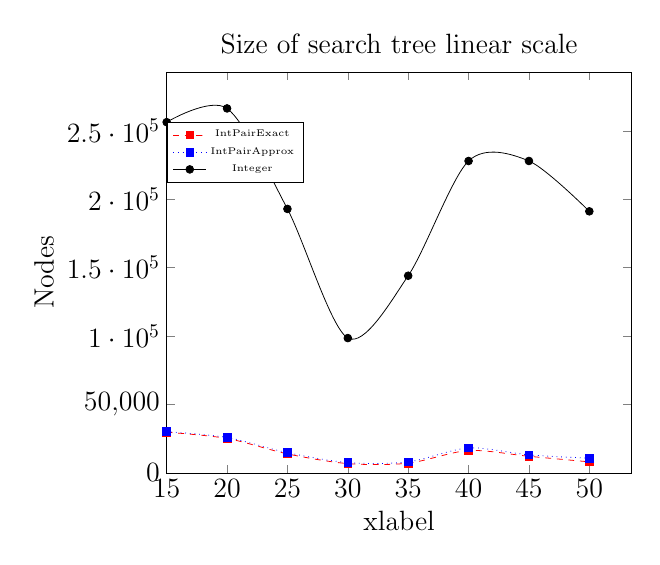
\begin{tikzpicture} [scale=0.7, font=\Large]
    \begin{axis}[
        title=Size of search tree linear scale,
        ylabel=Nodes,
        xtick=data,
        ymin=0, 
        xlabel=xlabel ]
      \addplot[smooth,mark=square*, mark options={solid},red, dashed]
      coordinates{ (15,29788) (20,25206) (25,13946) (30,6843) (35,7138) (40,16380) (45,12172) (50,8104)
      }; \label{ie_plot} \addlegendentry{IntPairExact}
      \addplot[smooth,mark=square*, mark options={solid},blue, dotted]
      coordinates{ (15,30142) (20,25936) (25,14840) (30,7617) (35,8090) (40,18266) (45,13224) (50,10748)
      }; \label{ia_plot} \addlegendentry{IntPairApprox}
      \addplot[smooth,mark=*,mark options={solid},black]
      coordinates{ (15,256300) (20,266332) (25,192912) (30,98546) (35,144086) (40,227922) (45,227934) (50,191140)
      }; \label{int_plot} \addlegendentry{Integer}
    \end{axis}
  \end{tikzpicture}
  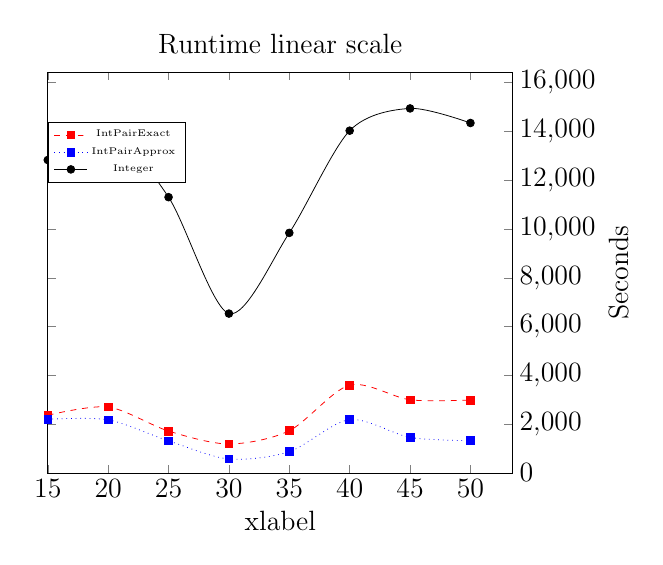
\begin{tikzpicture} [scale=0.7, font=\Large]
    \begin{axis}[
        yticklabel pos=right,
        xtick=data,
        title=Runtime linear scale,
        ylabel=Seconds,
        xlabel=xlabel,
        ymin=0, ]
      \addplot[smooth,mark=square*,mark options={solid},red, dashed]
      coordinates{ (15, 2366) (20, 2703) (25, 1718) (30, 1187) (35, 1731) (40, 3600) (45, 2999) (50, 2988)
      }; \label{IntPairExact Run}
      \addplot[smooth,mark=square*,mark options={solid},blue, dotted]
      coordinates{ (15, 2199) (20, 2177) (25, 1315) (30, 572) (35, 873) (40, 2188) (45, 1457) (50, 1324)
      }; \label{IntPairApprox Run}
      \addplot[smooth,mark=*,mark options={solid},black]
      coordinates{ (15, 12827) (20, 14021) (25, 11303) (30, 6532) (35, 9840) (40, 14029) (45, 14941) (50, 14344)
      }; \label{IntegerRun}
      \addlegendentry{IntPairExact}
      \addlegendentry{IntPairApprox}
      \addlegendentry{Integer}
    \end{axis}
  \end{tikzpicture}

  
\begin{tikzpicture}[scale=1.4]
    \draw[very thick] (-4,0) -- (4,0);
    \draw[draw=white] (-5,-0.2) -- (5,-0.2);
  \end{tikzpicture}


  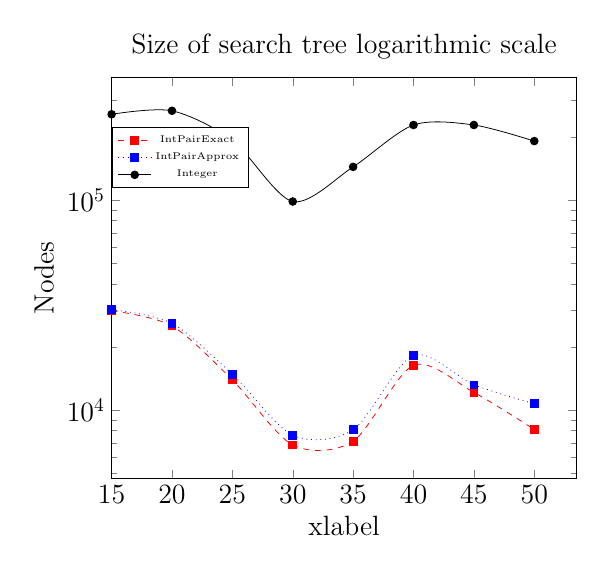
\begin{tikzpicture} [scale=0.7, font=\Large]
    \begin{semilogyaxis}[
        title=Size of search tree logarithmic scale,
        ylabel=Nodes,
        xtick=data,
        ymin=0, 
        xlabel=xlabel ]
     \addplot[smooth,mark=square*, mark options={solid},red, dashed]
      coordinates{ (15,29788) (20,25206) (25,13946) (30,6843) (35,7138) (40,16380) (45,12172) (50,8104)
      }; \label{ie_plot} \addlegendentry{IntPairExact}
      \addplot[smooth,mark=square*, mark options={solid},blue, dotted]
      coordinates{ (15,30142) (20,25936) (25,14840) (30,7617) (35,8090) (40,18266) (45,13224) (50,10748)
      }; \label{ia_plot} \addlegendentry{IntPairApprox}
      \addplot[smooth,mark=*,mark options={solid},black]
      coordinates{ (15,256300) (20,266332) (25,192912) (30,98546) (35,144086) (40,227922) (45,227934) (50,191140)
      }; \label{int_plot} \addlegendentry{Integer}

    \end{semilogyaxis}
  \end{tikzpicture}
  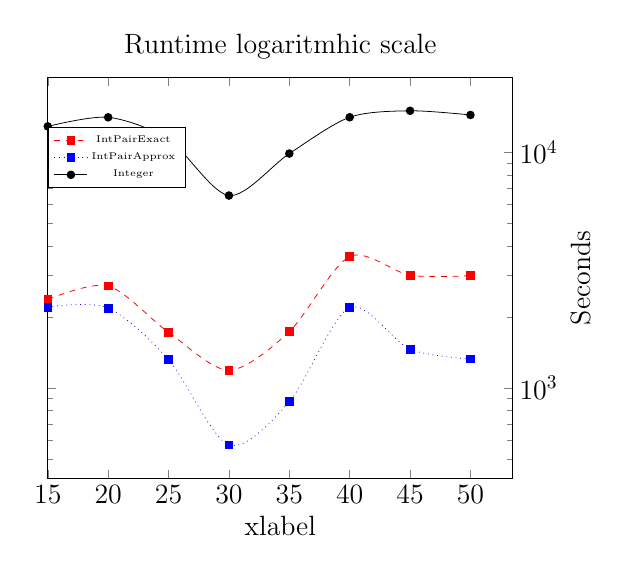
\begin{tikzpicture} [scale=0.7, font=\Large]
    \begin{semilogyaxis}[
        title=Runtime logaritmhic scale,
        yticklabel pos=right,
        xtick=data,
        ylabel=Seconds,
        xlabel=xlabel,
        ymin=0,  ]
      \addplot[smooth,mark=square*,mark options={solid},red, dashed]
      coordinates{ (15, 2366) (20, 2703) (25, 1718) (30, 1187) (35, 1731) (40, 3600) (45, 2999) (50, 2988)
      }; \label{IntPairExact Run}
      \addplot[smooth,mark=square*,mark options={solid},blue, dotted]
      coordinates{ (15, 2199) (20, 2177) (25, 1315) (30, 572) (35, 873) (40, 2188) (45, 1457) (50, 1324)
      }; \label{IntPairApprox Run}
      \addplot[smooth,mark=*,mark options={solid},black]
      coordinates{ (15, 12827) (20, 14021) (25, 11303) (30, 6532) (35, 9840) (40, 14029) (45, 14941) (50, 14344)
      }; \label{IntegerRun}
      \addlegendentry{IntPairExact}
      \addlegendentry{IntPairApprox}
      \addlegendentry{Integer}
    \end{semilogyaxis}
  \end{tikzpicture}
%  \input{}
%\end{figure}
  \caption{Varying the maximum cost per transition. The other parameters are fixed. Number of states=7, size of alphabet=10, and number of steps=7. The lack of an obvious dependence pattern between the x and y axis is because the maximum total cost also varies with the cost per transition.}\label{fig:cost}
 \end{figure}
